% Cella preprint. Build: tectonic main.tex   (or: xelatex/bibtex/xelatex x2)
% All numbers in the text come from numbers.tex, generated by
% scripts/make_figures.py from the project's artifacts.
\documentclass[11pt]{article}

\usepackage[a4paper,margin=2.3cm]{geometry}
\usepackage{fontspec}
\setmainfont{texgyretermes}[Extension=.otf, UprightFont=*-regular, BoldFont=*-bold,
  ItalicFont=*-italic, BoldItalicFont=*-bolditalic]
\setsansfont{texgyreheros}[Extension=.otf, UprightFont=*-regular, BoldFont=*-bold,
  ItalicFont=*-italic, BoldItalicFont=*-bolditalic]
\usepackage{amsmath}
\usepackage{microtype}
\usepackage{graphicx}
\usepackage{booktabs}
\usepackage{tabularx}
\usepackage{array}
\usepackage[table]{xcolor}
\usepackage{caption}
\usepackage{subcaption}
\usepackage{tikz}
\usetikzlibrary{arrows.meta,positioning,fit,backgrounds,calc}
\usepackage[numbers,sort&compress]{natbib}
\usepackage{authblk}
\usepackage[mathlines]{lineno}
\usepackage{enumitem}
\usepackage{xurl}
\usepackage[colorlinks=true,linkcolor=accent,citecolor=accent,urlcolor=accent]{hyperref}

\definecolor{accent}{HTML}{1C5CAB}
\definecolor{lowprev}{HTML}{B0413E}
\definecolor{boxfill}{HTML}{F2F6FB}
\definecolor{boxline}{HTML}{86B6EF}
\definecolor{ink2}{HTML}{52514E}

\captionsetup{font=small,labelfont=bf,labelsep=period}
\setlength{\parskip}{0.35em}
\renewcommand{\Authfont}{\normalsize}
\renewcommand{\Affilfont}{\small}

% Generated by preprint/scripts/make_figures.py - do not edit by hand.
\newcommand{\calConfFrac}{32\%}
\newcommand{\calDevPrecConf}{0.68}
\newcommand{\calMarginMax}{0.25}
\newcommand{\calMarginMin}{0.05}
\newcommand{\calNConf}{73}
\newcommand{\calNRest}{158}
\newcommand{\calPrecConf}{0.67}
\newcommand{\calPrecConfCI}{0.56--0.77}
\newcommand{\calPrecRest}{0.29}
\newcommand{\calPrecRestCI}{0.23--0.37}
\newcommand{\exportJsonMB}{23.5}
\newcommand{\exportMeanMB}{16.9}
\newcommand{\exportPctMB}{7.6}
\newcommand{\gateAdipoGatedRank}{10}
\newcommand{\gateAdipoRawRank}{107}
\newcommand{\gateFracAll}{58\%}
\newcommand{\gateFracTopFive}{27\%}
\newcommand{\gateGobletGatedRank}{10}
\newcommand{\gateGobletRawRank}{95}
\newcommand{\gateMajority}{253}
\newcommand{\gateNTypes}{399}
\newcommand{\gateRho}{-0.59}
\newcommand{\gateRhoP}{2.4\times10^{-39}}
\newcommand{\invCalCirc}{0.177}
\newcommand{\invCalP}{0.0025}
\newcommand{\invCalRes}{0.092}
\newcommand{\invMulti}{49}
\newcommand{\invNCirc}{22}
\newcommand{\invNExcluded}{7}
\newcommand{\invNPairsLL}{6}
\newcommand{\invNPairsPP}{27}
\newcommand{\invNRes}{8}
\newcommand{\invNStab}{28}
\newcommand{\invNullLL}{0.179}
\newcommand{\invNullPP}{0.101}
\newcommand{\invNullSD}{0.064}
\newcommand{\invNullSDRange}{0.03--0.14}
\newcommand{\invPerNCirc}{14}
\newcommand{\invPerP}{0.059}
\newcommand{\invRawP}{4.6\times10^{-5}}
\newcommand{\invRhoCells}{-0.02}
\newcommand{\invRhoCellsP}{0.90}
\newcommand{\invRhoStab}{-0.15}
\newcommand{\invRhoStabP}{0.45}
\newcommand{\invSensNHaem}{20}
\newcommand{\invSensP}{0.0039}
\newcommand{\invTierOne}{30}
\newcommand{\invTierTwo}{12}
\newcommand{\lkAzExprTopOne}{76\%}
\newcommand{\lkAzHyperTopOne}{78\%}
\newcommand{\lkAzN}{58}
\newcommand{\lkAzWmeanTopOne}{57\%}
\newcommand{\lkCMExprTopOne}{50\%}
\newcommand{\lkCMHyperTopOne}{58\%}
\newcommand{\lkCMN}{150}
\newcommand{\lkCMWmeanTopOne}{35\%}
\newcommand{\lkDev}{150}
\newcommand{\lkDevEspecMRR}{0.62}
\newcommand{\lkDevEspecTopFive}{79\%}
\newcommand{\lkDevEspecTopOneX}{48\%}
\newcommand{\lkDevExprMRR}{0.63}
\newcommand{\lkDevExprTopFive}{77\%}
\newcommand{\lkDevExprTopOne}{50\%}
\newcommand{\lkDevExprTopOneX}{50\%}
\newcommand{\lkDevHyperMRR}{0.65}
\newcommand{\lkDevHyperTopFive}{73\%}
\newcommand{\lkDevHyperTopOneX}{58\%}
\newcommand{\lkDevWmeanTopOne}{35\%}
\newcommand{\lkDisc}{57}
\newcommand{\lkDiscRev}{5}
\newcommand{\lkExprTopFive}{73\%}
\newcommand{\lkExprTopOne}{40\%}
\newcommand{\lkExprTopOneCI}{34--46\%}
\newcommand{\lkHybridDisc}{45}
\newcommand{\lkHybridDiscRev}{28}
\newcommand{\lkHybridMcNemarP}{0.06}
\newcommand{\lkHybridTopFive}{58\%}
\newcommand{\lkHybridTopOne}{32\%}
\newcommand{\lkHyperDisc}{34}
\newcommand{\lkHyperDiscRev}{23}
\newcommand{\lkHyperMcNemarP}{0.18}
\newcommand{\lkHyperTopFive}{55\%}
\newcommand{\lkHyperTopOne}{35\%}
\newcommand{\lkIndependent}{381}
\newcommand{\lkLibExprGtWmean}{4}
\newcommand{\lkLibHyperGtExpr}{3}
\newcommand{\lkMcNemarP}{3.1\times10^{-12}}
\newcommand{\lkOvExprTopOne}{66\%}
\newcommand{\lkOvWmeanTopOne}{32\%}
\newcommand{\lkOverlap}{161}
\newcommand{\lkPgExprTopOne}{25\%}
\newcommand{\lkPgHyperTopOne}{32\%}
\newcommand{\lkPgN}{57}
\newcommand{\lkPgWmeanTopOne}{5\%}
\newcommand{\lkPseudoTopFive}{24\%}
\newcommand{\lkPseudoTopOne}{5\%}
\newcommand{\lkResolved}{829}
\newcommand{\lkScored}{542}
\newcommand{\lkSubFiveExpr}{38\%}
\newcommand{\lkSubFiveWmean}{17\%}
\newcommand{\lkSubTenExpr}{30\%}
\newcommand{\lkSubTenWmean}{14\%}
\newcommand{\lkSubThreeExpr}{33\%}
\newcommand{\lkSubThreeWmean}{16\%}
\newcommand{\lkTSExprTopOne}{29\%}
\newcommand{\lkTSHyperTopOne}{16\%}
\newcommand{\lkTSN}{116}
\newcommand{\lkTSWmeanTopOne}{3\%}
\newcommand{\lkTerms}{3{,}764}
\newcommand{\lkTest}{231}
\newcommand{\lkWgatedTopFive}{47\%}
\newcommand{\lkWgatedTopOne}{22\%}
\newcommand{\lkWgenezTopFive}{49\%}
\newcommand{\lkWgenezTopOne}{25\%}
\newcommand{\lkWmeanTopFive}{32\%}
\newcommand{\lkWmeanTopOne}{17\%}
\newcommand{\lkWmeanTopOneCI}{12--23\%}
\newcommand{\maxModelGenes}{10{,}396}
\newcommand{\minModelGenes}{5{,}529}
\newcommand{\nCLTerms}{145}
\newcommand{\nCells}{3.69}
\newcommand{\nDatasets}{38}
\newcommand{\nExportFiles}{1{,}339}
\newcommand{\nLabels}{399}
\newcommand{\nMultiOrganTerms}{49}
\newcommand{\nOrgans}{12}
\newcommand{\pnLFiveLfcDiff}{-0.016}
\newcommand{\pnLFiveLfcP}{0.022}
\newcommand{\pnLFiveLfcPHolm}{0.22}
\newcommand{\pnLFiveLfcWins}{18/48}
\newcommand{\pnLFiveRawDiff}{+0.008}
\newcommand{\pnLFiveRawP}{5.4\times10^{-4}}
\newcommand{\pnLFiveRawPHolm}{0.0076}
\newcommand{\pnLFiveRawWins}{35/48}
\newcommand{\pnLFiveWilcDiff}{-0.021}
\newcommand{\pnLFiveWilcP}{0.0093}
\newcommand{\pnLFiveWilcPHolm}{0.12}
\newcommand{\pnLFiveWilcWins}{19/48}
\newcommand{\pnLTenLfcDiff}{-0.009}
\newcommand{\pnLTenLfcP}{0.77}
\newcommand{\pnLTenLfcPHolm}{1}
\newcommand{\pnLTenLfcWins}{28/48}
\newcommand{\pnLTenRawDiff}{+0.014}
\newcommand{\pnLTenRawP}{3.8\times10^{-4}}
\newcommand{\pnLTenRawPHolm}{0.0058}
\newcommand{\pnLTenRawWins}{36/48}
\newcommand{\pnLTenWilcDiff}{-0.011}
\newcommand{\pnLTenWilcP}{0.45}
\newcommand{\pnLTenWilcPHolm}{1}
\newcommand{\pnLTenWilcWins}{26/48}
\newcommand{\pnLThreeLfcDiff}{-0.018}
\newcommand{\pnLThreeLfcP}{0.029}
\newcommand{\pnLThreeLfcPHolm}{0.26}
\newcommand{\pnLThreeLfcWins}{18/48}
\newcommand{\pnLThreeRawDiff}{+0.011}
\newcommand{\pnLThreeRawP}{3.0\times10^{-6}}
\newcommand{\pnLThreeRawPHolm}{5.7\times10^{-5}}
\newcommand{\pnLThreeRawWins}{39/48}
\newcommand{\pnLThreeWilcDiff}{-0.034}
\newcommand{\pnLThreeWilcP}{7.4\times10^{-6}}
\newcommand{\pnLThreeWilcPHolm}{1.3\times10^{-4}}
\newcommand{\pnLThreeWilcWins}{11/48}
\newcommand{\pnLTwentyLfcDiff}{+0.002}
\newcommand{\pnLTwentyLfcP}{0.073}
\newcommand{\pnLTwentyLfcPHolm}{0.51}
\newcommand{\pnLTwentyLfcWins}{32/48}
\newcommand{\pnLTwentyRawDiff}{+0.024}
\newcommand{\pnLTwentyRawP}{1.4\times10^{-6}}
\newcommand{\pnLTwentyRawPHolm}{2.8\times10^{-5}}
\newcommand{\pnLTwentyRawWins}{39/48}
\newcommand{\pnLTwentyWilcDiff}{+0.001}
\newcommand{\pnLTwentyWilcP}{0.084}
\newcommand{\pnLTwentyWilcPHolm}{0.51}
\newcommand{\pnLTwentyWilcWins}{32/48}
\newcommand{\pnMFiveLfcDiff}{+0.019}
\newcommand{\pnMFiveLfcP}{0.039}
\newcommand{\pnMFiveLfcPHolm}{0.31}
\newcommand{\pnMFiveLfcWins}{32/48}
\newcommand{\pnMFiveRawDiff}{+0.025}
\newcommand{\pnMFiveRawP}{6.9\times10^{-8}}
\newcommand{\pnMFiveRawPHolm}{1.5\times10^{-6}}
\newcommand{\pnMFiveRawWins}{39/48}
\newcommand{\pnMFiveWilcDiff}{-0.009}
\newcommand{\pnMFiveWilcP}{1}
\newcommand{\pnMFiveWilcPHolm}{1}
\newcommand{\pnMFiveWilcWins}{28/48}
\newcommand{\pnMTenLfcDiff}{+0.032}
\newcommand{\pnMTenLfcP}{2.4\times10^{-4}}
\newcommand{\pnMTenLfcPHolm}{0.0039}
\newcommand{\pnMTenLfcWins}{37/48}
\newcommand{\pnMTenRawDiff}{+0.051}
\newcommand{\pnMTenRawP}{6.4\times10^{-12}}
\newcommand{\pnMTenRawPHolm}{1.5\times10^{-10}}
\newcommand{\pnMTenRawWins}{44/48}
\newcommand{\pnMTenWilcDiff}{+0.004}
\newcommand{\pnMTenWilcP}{0.16}
\newcommand{\pnMTenWilcPHolm}{0.81}
\newcommand{\pnMTenWilcWins}{31/48}
\newcommand{\pnMThreeLfcDiff}{+0.027}
\newcommand{\pnMThreeLfcP}{0.0093}
\newcommand{\pnMThreeLfcPHolm}{0.12}
\newcommand{\pnMThreeLfcWins}{33/48}
\newcommand{\pnMThreeRawDiff}{+0.015}
\newcommand{\pnMThreeRawP}{9.4\times10^{-8}}
\newcommand{\pnMThreeRawPHolm}{2.0\times10^{-6}}
\newcommand{\pnMThreeRawWins}{39/48}
\newcommand{\pnMThreeWilcDiff}{-0.002}
\newcommand{\pnMThreeWilcP}{0.37}
\newcommand{\pnMThreeWilcPHolm}{1}
\newcommand{\pnMThreeWilcWins}{30/48}
\newcommand{\pnMTwentyLfcDiff}{+0.036}
\newcommand{\pnMTwentyLfcP}{1.5\times10^{-4}}
\newcommand{\pnMTwentyLfcPHolm}{0.0025}
\newcommand{\pnMTwentyLfcWins}{35/48}
\newcommand{\pnMTwentyRawDiff}{+0.081}
\newcommand{\pnMTwentyRawP}{3.1\times10^{-13}}
\newcommand{\pnMTwentyRawPHolm}{7.3\times10^{-12}}
\newcommand{\pnMTwentyRawWins}{47/48}
\newcommand{\pnMTwentyWilcDiff}{+0.016}
\newcommand{\pnMTwentyWilcP}{0.018}
\newcommand{\pnMTwentyWilcPHolm}{0.2}
\newcommand{\pnMTwentyWilcWins}{30/48}
\newcommand{\pnMWilcOtherMinPHolm}{0.81}
\newcommand{\pnNTests}{24}
\newcommand{\pnOrgans}{12}
\newcommand{\pnRawMaxPHolm}{0.0076}
\newcommand{\pnSizeGated}{298}
\newcommand{\pnSizeWilc}{218}
\newcommand{\pnSplits}{48}
\newcommand{\pnSplitsPerOrgan}{4}
\newcommand{\pnWilcOrgansBetter}{5}

% Static-vs-server equivalence, from `npx tsx web/scripts/check-static.ts`
% (run 2026-10-14 against the live API with 120 benchmark queries + 6 built-in
% signatures). Re-run that script and update these values if the data change.
\newcommand{\eqQueries}{126}
\newcommand{\eqSameTop}{124}
\newcommand{\eqTies}{2}
\newcommand{\eqSameConf}{126/126}
\newcommand{\eqMaxDiff}{0.0013}
\newcommand{\eqGeneDiff}{0.002}
\newcommand{\eqSigDiff}{0.001}
\newcommand{\eqExportMin}{1}


\newcommand{\gene}[1]{\textit{#1}}
% Expandable input for generated table rows (plain \input breaks \bottomrule).
\makeatletter\newcommand{\tablerows}[1]{\@@input #1 }\makeatother
\newcommand{\cella}{Cella}

\title{\textbf{Cella: a serverless web resource for querying discriminative cell-type identity across twelve human organ atlases}}
\author[1,2]{Md.~Jubayer Hossain\thanks{Correspondence: \href{mailto:contact.jubayerhossain@gmail.com}{contact.jubayerhossain@gmail.com}}}
\affil[1]{Center for Health Innovation, Research, Action, and Learning -- Bangladesh, Dhaka, Bangladesh}
\affil[2]{DeepBio, Dhaka, Bangladesh}
\date{Preprint, \today}

\begin{document}
\maketitle

\begin{abstract}
\noindent
Supervised cell-type classifiers trained on curated single-cell atlases learn, for every cell type, a weight for every gene, yet these weights are distributed only inside model files. We present \cella{}, an open web resource that turns the logistic-regression classifiers and pseudobulk expression of the CellTypist organ atlases (\nOrgans{} organs, \nDatasets{} datasets, \nCells{} million cells, \nLabels{} organ-specific labels harmonised to \nCLTerms{} Cell Ontology terms) into five interactive tools: an organ browser, a discriminative marker atlas, a cross-organ fingerprint explorer, a cell-type relationship graph and a gene-signature lookup. Building the resource exposed a pitfall in reading classifier coefficients directly: because genes are standardised before fitting, genes detected in almost no cells acquire large weights for rare classes, and \gateFracAll{} of raw top-25 positive coefficients were genes expressed in fewer than 10\% of the cell type's own cells. Gating markers on expression prevalence restored canonical markers and, on \pnSplits{} leave-one-dataset-out splits, produced marker panels on par with Wilcoxon differential expression and better than raw coefficients. We benchmarked the signature lookup against \lkScored{} external marker sets with method selection and evaluation on separate libraries; ranking by the fraction of cells expressing the query placed the correct cell type first for \lkExprTopOne{} of held-out queries, against \lkWmeanTopOne{} for mean classifier weight, so classifier weights are used to explain hits rather than to rank them. A calibrated confidence call and an ontology-aware treatment of related cell types accompany every lookup. \cella{} runs entirely in the browser from pre-computed files, so it is hosted at no cost and can be archived with its code; the same codebase also serves a FastAPI backend. \cella{} is available at \url{https://mdjubayerhossain.com/cella/} and the source at \url{https://github.com/hossainlab/cella}.
\end{abstract}

\noindent\textbf{Keywords:} single-cell RNA sequencing; cell-type annotation; marker genes; CellTypist; Cell Ontology; web server

\linenumbers

\section{Introduction}

Large single-cell reference atlases have shifted cell-type annotation from manual inspection of clusters towards automated label transfer \cite{regev2017,abdelaal2019}. Among the most widely used tools is CellTypist, which fits regularised logistic-regression classifiers to harmonised reference data and was first applied to immune cells across sixteen human tissues \cite{dominguez2022}. Its successor work harmonised cell-type labels across Human Cell Atlas datasets and released organ-level atlases with matching classifiers \cite{xu2023,celltypistorgans}. Each of these classifiers is, in effect, a matrix with one weight per gene and cell type, describing which genes the model uses to separate that cell type from its neighbours in the same organ.

Atlas portals such as CZ CELLxGENE Discover \cite{cellxgene2025} and reference-mapping services such as Azimuth \cite{hao2021} make expression and annotation accessible at scale, and curated databases such as CellMarker \cite{cellmarker2023} and PanglaoDB \cite{panglaodb2019} catalogue literature markers. The classifier weights themselves, however, are distributed inside serialised model files. Reading them requires programming, and comparing them across organs requires harmonising labels, aligning gene spaces and handling cell types that are annotated at different granularities in different organs. Questions that the weights could answer directly---which genes define a cell type in a given organ, which of those are shared across organs, and which cell type a list of genes points to---are therefore not easily asked by most users.

We built \cella{} to make these questions answerable in a browser. In doing so we found that classifier coefficients cannot be read naively as marker rankings, and that a resource built on them needs to be benchmarked rather than assumed to work. This article describes the resource, the prevalence gating that makes its marker lists usable, two benchmarks on held-out data and external marker sets that determined how its tools score, a cross-organ use case, and a serverless deployment that keeps the resource free to host and simple to archive.

\section{Materials and methods}

\subsection{Data sources and harmonisation}

We used the twelve adult human organ atlases distributed by CellTypist (blood, bone marrow, heart, hippocampus, intestine, kidney, liver, lung, lymph node, pancreas, skeletal muscle and spleen) and their pretrained classifiers \cite{xu2023,celltypistorgans}. Each atlas provides cell-level metadata, including a curated annotation on which the classifier was trained and a Cell Ontology label; each classifier provides a coefficient matrix over its own feature set (\minModelGenes{}--\maxModelGenes{} genes) together with the standard scaler fitted to its training data. Downloads are scripted and recorded with checksums. Curated labels were mapped to Cell Ontology identifiers \cite{diehl2016} by exact label, then synonym, then a single manual override, which resolved all \nCLTerms{} terms used across the \nLabels{} organ-specific labels; \nMultiOrganTerms{} terms occur in two or more organs. For every organ we computed a pseudobulk summary per curated label, namely the mean log-normalised expression and the fraction of cells with non-zero expression, streaming the expression matrix in blocks so that no atlas is loaded into memory whole.

\subsection{Prevalence-gated discriminative markers}

For a curated label $c$ in organ $o$, let $\beta_{c,g}$ be the classifier coefficient of gene $g$, $p_{c,g}$ the fraction of cells of $c$ expressing $g$, and $\bar p_{-c,g} = \max_{c' \neq c} p_{c',g}$ the highest such fraction among the other labels of the organ. Positive markers are the top $n$ genes by $\beta_{c,g}$ among those with $p_{c,g} \geq \tau$; negative markers are the bottom $n$ genes by $\beta_{c,g}$ among those with $\bar p_{-c,g} \geq \tau$, because a negative weight is informative only if some other cell type in the organ expresses the gene. We used $n = 25$ and $\tau = 0.1$; setting $\tau = 0$ recovers the raw coefficient ranking. For each Cell Ontology term, the marker atlas reports genes that are top positive markers in every organ where the term occurs (universal core), genes shared by two or more organs, and genes specific to a single organ (tissue-adapted).

\subsection{Relationship graph and organ-level layers}

The relationship graph links Cell Ontology terms whose classifier-weight vectors are similar. A term's vector is the mean of its organ-level weight rows over the union of genes (absent genes set to zero); each term keeps up to six neighbours with cosine similarity of at least 0.15, and node positions come from a seeded spring layout so that the graph is identical on every load. The organ browser adds the atlas UMAP embedding (downsampled to 25{,}000 cells), transcription-factor activities inferred with the univariate linear model of decoupleR \cite{badia2022} over CollecTRI regulons \cite{mullerdott2023}, gene-set activities for six MSigDB collections (release 2023.2.Hs, including the hallmark collection \cite{liberzon2015}), and ligand--receptor scores computed as the product of mean ligand and receptor expression between labels, using the consensus resource of LIANA \cite{dimitrov2022} and requiring each partner to be expressed in at least 10\% of cells.

\subsection{Gene-signature lookup}

Given a query gene set $Q$, \cella{} scores every curated label $c$ in every organ $o$ by
\begin{equation}
S(c) = \frac{1}{|Q_o|} \sum_{g \in Q_o} p_{c,g},
\end{equation}
where $Q_o$ is the part of the query present in organ $o$'s vocabulary, and ranks labels across all organs. Each hit reports, for its most widely expressed query genes, both $p_{c,g}$ and the classifier weight $\beta_{c,g}$. A lookup is called confident when the best score is at least 0.3 and leads the best score of any cell type that is neither the same term nor a close ontology relative by at least 10\% of the best score. Close relatives are specific parents (ancestors of at most three atlas terms) and, for terms with at most five atlas descendants, their descendants; generic terms such as \emph{cell} therefore have no close relatives. The scoring rule and both thresholds were chosen on a development library only, as described next.

\subsection{Benchmark of signature lookup against external marker sets}

Queries were cell-type marker sets curated independently of CellTypist, obtained from four libraries distributed by Enrichr \cite{kuleshov2016}: Tabula Sapiens \cite{tabulasapiens2022}, Azimuth 2023, CellMarker 2024 and PanglaoDB Augmented 2021 (\lkTerms{} terms in total). We kept human terms from tissues covered by the atlases, resolved their cell-type names to Cell Ontology identifiers (\lkResolved{} terms), and scored a query only if an atlas term could answer it and the query term was specific enough to be informative (at most five atlas descendants), leaving \lkScored{} queries. Queries whose source data overlap the CellTypist training data (Tabula Sapiens bone marrow, muscle and spleen; Azimuth lung, heart and kidney) were analysed separately (\lkOverlap{} queries), leaving \lkIndependent{} independent queries.

Each method ranks Cell Ontology terms by the best score of any curated label annotated with the term, so the organ is not given. A hit is correct if it is the query term, one of its descendants, or a specific ancestor; ties count half a rank so that methods producing many ties are not favoured. We compared nine scoring rules: mean classifier weight; mean weight after prevalence gating; per-gene z-scored weights with and without gating; the classifier's own decision function evaluated on a pseudo-cell expressing only the query genes; mean fraction expressing; mean per-gene z-scored expression; a hypergeometric test against the gated top-25 marker lists; and the average of the z-scored gated weight and expression scores. Methods and thresholds were selected on CellMarker (\lkDev{} independent queries) and evaluated on the other three libraries (\lkTest{} queries). We report top-1 and top-5 accuracy with 95\% bootstrap intervals (2{,}000 resamples), mean reciprocal rank, and an exact McNemar test on paired top-1 outcomes. To mimic short pasted lists, each query was also subsampled to 3, 5 and 10 genes in five random draws.

\subsection{Benchmark of marker panels on held-out datasets}

To ask whether gated coefficients make better marker panels than differential expression, we held out each source dataset of each organ in turn (\pnSplits{} splits over \pnOrgans{} organs). Training cells came from the remaining datasets, capped at 500 per label; test cells came from the held-out dataset, capped at 300 per label, for labels with at least 20 test cells and 50 training cells. Within each split, and on training cells only, we retrained CellTypist with its default settings on the released model's feature set and ranked markers by raw coefficient, by gated coefficient, by Wilcoxon rank-sum score in Scanpy \cite{wolf2018} (one label versus the rest, restricted to the same feature set) and by gated log fold change. For $k \in \{3, 5, 10, 20\}$ markers per label we measured macro-F1 on the held-out cells in two ways: a classifier-free assignment of each cell to the label whose own $k$ markers have the highest mean z-score, and a fresh multinomial logistic regression \cite{pedregosa2011} trained on the union of all labels' markers. Differences between methods were tested with paired Wilcoxon signed-rank tests across splits.

\subsection{Cross-organ invariance of discriminative identity}

For each Cell Ontology term annotated in at least two organs, we compared its weight vectors between every pair of organs by cosine similarity over the genes shared by the two models (labels sharing a term within an organ were averaged, weighted by cell count). The null for an organ pair is the distribution of cosines between mismatched cell types of the same two organs, and the calibrated invariance of a term is the mean, over its organ pairs, of the cosine minus that pair's null mean. Terms that are ontology ancestors of another annotated term were scored only over the organs in which no descendant was annotated separately, or excluded when fewer than two such organs remained. Coefficient reproducibility was estimated by retraining each organ's classifier on five disjoint, equally sized folds of 200 cells per label and computing the mean pairwise cosine of the replicate vectors.

\subsection{Implementation and deployment}

The offline pipeline is written in Python and writes Parquet artifacts; a FastAPI service exposes them, and a Next.js application provides the interface. The interface can be built in two modes from the same code. In server mode it queries the FastAPI service. In static mode, used for the public site, a command (\texttt{cella export}) calls every endpoint whose inputs form a finite set---each organ, cell type, graph edge and gene-set collection---on the FastAPI application in-process and saves the responses (\nExportFiles{} files, \exportJsonMB{}\,MB), and writes per-organ expression tables in compact form: fraction expressing as 8-bit and mean expression as 16-bit integers scaled to the organ maximum, compressed (\exportPctMB{}\,MB and \exportMeanMB{}\,MB). The signature lookup, gene and signature queries and the corresponding UMAP figures are re-implemented in the browser against these tables, and a test script compares them with the live service. The static build is deployed by a continuous-integration workflow to GitHub Pages; no server, account or login is involved.

\section{Results}

\subsection{Overview of the resource}

\cella{} is organised around five tools that share the harmonised cell-type registry (Figure~\ref{fig:pipeline}, Table~\ref{tab:tools}). The organ browser summarises each atlas (composition, UMAP, gene and signature views, transcription-factor and pathway activity, and ligand--receptor interactions). The marker atlas lists the gated discriminative markers of a cell type in every organ where it occurs and separates the universal core from organ-specific markers (Figure~\ref{fig:interface}a). The fingerprint explorer shows signed weights side by side across organs, the relationship graph links related cell types across organs, and the signature lookup ranks cell types for a pasted gene list (Figure~\ref{fig:interface}b).

\begin{figure}[t]
\centering
\resizebox{\textwidth}{!}{%
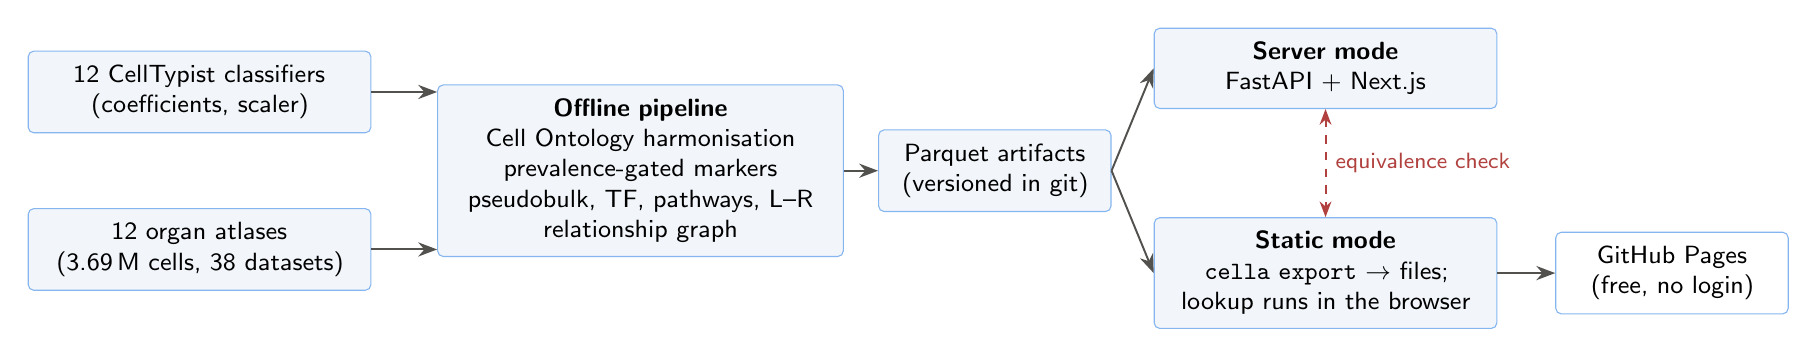
\begin{tikzpicture}[
  font=\sffamily\small,
  box/.style={draw=boxline, fill=boxfill, rounded corners=2pt, align=center, inner sep=5pt},
  arr/.style={-{Stealth[length=2.4mm]}, draw=ink2, line width=0.7pt}]
  \node[box, text width=4.0cm] (models) at (0, 1.0) {12 CellTypist classifiers\\(coefficients, scaler)};
  \node[box, text width=4.0cm] (atlas) at (0,-1.0) {12 organ atlases\\(\nCells{}\,M cells, \nDatasets{} datasets)};
  \node[box, text width=4.8cm] (pipe) at (5.6, 0) {\textbf{Offline pipeline}\\Cell Ontology harmonisation\\prevalence-gated markers\\pseudobulk, TF, pathways, L--R\\relationship graph};
  \node[box, text width=2.6cm] (art) at (10.1, 0) {Parquet artifacts\\(versioned in git)};
  \node[box, text width=4.0cm] (server) at (14.3, 1.3) {\textbf{Server mode}\\FastAPI + Next.js};
  \node[box, text width=4.0cm] (static) at (14.3,-1.3) {\textbf{Static mode}\\\texttt{cella export} $\rightarrow$ files;\\lookup runs in the browser};
  \node[box, text width=2.6cm, fill=white] (pages) at (18.7,-1.3) {GitHub Pages\\(free, no login)};
  \draw[arr] (models.east) -- (pipe.west |- models.east);
  \draw[arr] (atlas.east) -- (pipe.west |- atlas.east);
  \draw[arr] (pipe) -- (art);
  \draw[arr] (art.east) -- (server.west);
  \draw[arr] (art.east) -- (static.west);
  \draw[arr] (static) -- (pages);
  \draw[{Stealth[length=2mm]}-{Stealth[length=2mm]}, draw=lowprev, dashed, line width=0.7pt]
    (server.south) -- node[right, text=lowprev, font=\sffamily\footnotesize]{equivalence check} (static.north);
\end{tikzpicture}}
\caption{\textbf{Architecture of \cella{}.} An offline pipeline turns the CellTypist classifiers and atlases into versioned Parquet artifacts. The same interface is built either against a FastAPI service (server mode) or against pre-computed files with in-browser computation for free-text queries (static mode, used for the public site); a test compares the two modes' answers.}
\label{fig:pipeline}
\end{figure}

\begin{table}[t]
\centering
\small
\caption{\textbf{The five tools of \cella{}.} All tools share the Cell Ontology registry of \nCLTerms{} terms.}
\label{tab:tools}
\begin{tabularx}{\textwidth}{@{}>{\raggedright\arraybackslash}p{2.6cm}>{\raggedright\arraybackslash}X>{\raggedright\arraybackslash}X@{}}
\toprule
Tool & Question answered & Data used \\
\midrule
Organ browser & What does this organ contain, and how is a gene or signature distributed across its cell types? & Atlas metadata, UMAP, pseudobulk, TF and pathway activities, ligand--receptor scores \\
Marker atlas & Which genes define this cell type in each organ, and which are shared? & Gated positive and negative coefficients \\
Fingerprint explorer & How does the weight of each defining gene change across organs? & Signed coefficients per organ \\
Relationship graph & Which cell types, in any organ, are defined similarly? & Cosine similarity of term-level weight vectors \\
Signature lookup & Which cell type does this gene list describe, and how confidently? & Fraction expressing (ranking); coefficients (evidence) \\
\bottomrule
\end{tabularx}
\end{table}

\begin{figure}[t]
\centering
\begin{subfigure}{\textwidth}
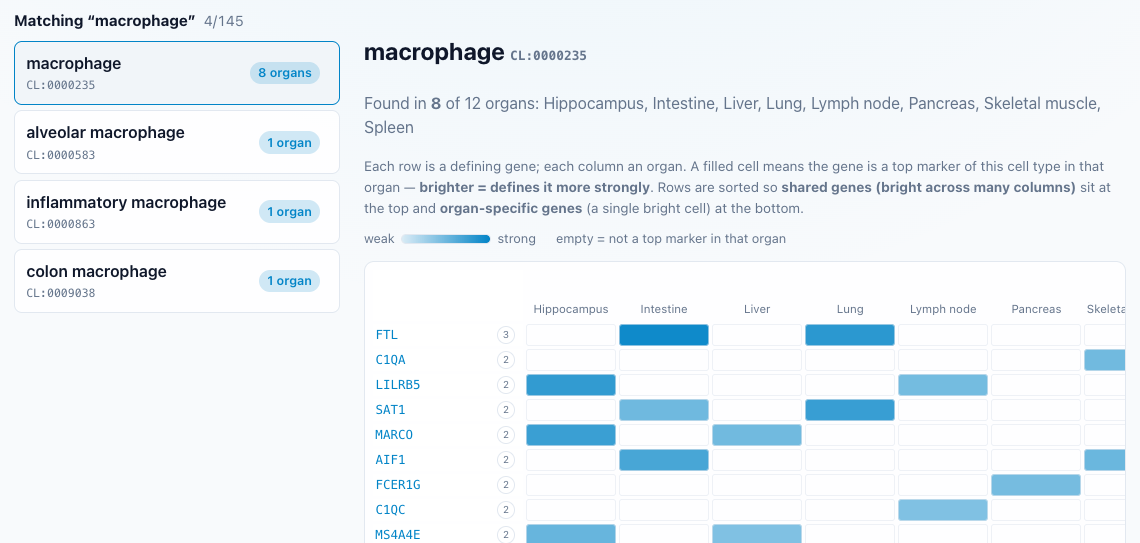
\includegraphics[width=\linewidth]{figures/fig1_atlas.png}
\caption{}
\end{subfigure}\\[0.4em]
\begin{subfigure}{\textwidth}
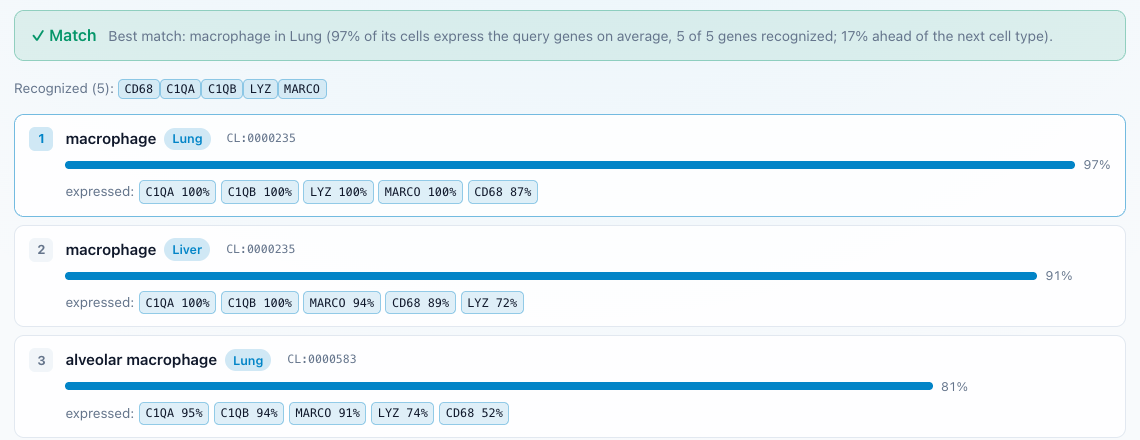
\includegraphics[width=\linewidth]{figures/fig1_lookup.png}
\caption{}
\end{subfigure}
\caption{\textbf{The \cella{} interface (public static site).} (\textbf{a}) Marker atlas for \emph{macrophage}, found in eight organs: each row is a gated discriminative gene and each column an organ; shared genes are listed first. (\textbf{b}) Signature lookup for \gene{CD68}, \gene{C1QA}, \gene{C1QB}, \gene{LYZ} and \gene{MARCO}: ranked hits with the fraction of cells expressing each gene; the alveolar macrophage hit is an ontology relative of the top hit and does not count against the confident call.}
\label{fig:interface}
\end{figure}

\subsection{Raw classifier coefficients are dominated by rarely detected genes}

Ranking each label's genes by raw coefficient produced marker lists that were frequently implausible. Across the \gateNTypes{} organ-specific labels, \gateFracAll{} of the raw top-25 positive markers, and \gateFracTopFive{} of the top five, were genes expressed in fewer than 10\% of the label's own cells; for \gateMajority{} labels such genes made up more than half of the list (Figure~\ref{fig:gating}a). The problem concentrated in rare labels (Spearman $\rho = \gateRho{}$ between the contaminated fraction and the number of training cells, $P = \gateRhoP{}$; Figure~\ref{fig:gating}b). This is consistent with the classifiers standardising each gene before fitting: a gene detected in a handful of cells has a small standard deviation, takes large standardised values in the few cells where it appears, and can carry a large coefficient that helps separate a small class without being a marker of it. Lung goblet cells, for example, ranked \gene{FOXP3} among their top raw markers, and heart adipocytes ranked the natural-killer receptor \gene{CD244} (Table~\ref{tab:gating}). Prevalence gating removed these genes and recovered canonical markers such as \gene{MUC5AC} for goblet cells and \gene{PPARG} for adipocytes, while leaving well-represented labels such as alveolar macrophages unchanged.

\begin{figure}[t]
\centering
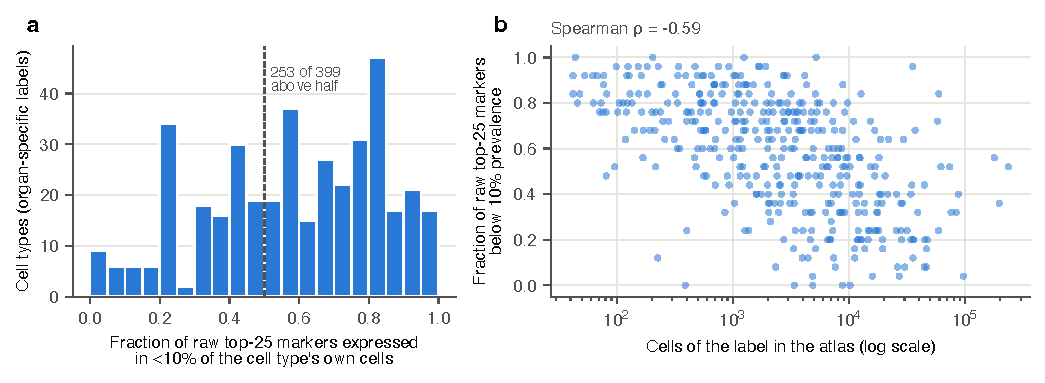
\includegraphics[width=\textwidth]{figures/fig2_gating.pdf}
\caption{\textbf{Raw classifier coefficients favour rarely detected genes.} (\textbf{a}) For each of the \gateNTypes{} organ-specific labels, the fraction of its raw top-25 positive markers that are expressed in fewer than 10\% of its own cells. (\textbf{b}) The same fraction against the number of training cells for the label.}
\label{fig:gating}
\end{figure}

\begin{table}[t]
\centering
\scriptsize
\caption{\textbf{Top positive markers before and after prevalence gating.} Genes expressed in fewer than 10\% of the label's cells are shown in \textcolor{lowprev}{red}.}
\label{tab:gating}
\begin{tabularx}{\textwidth}{@{}llXX@{}}
\toprule
Organ & Label & Raw coefficient ranking (top 6) & Gated ranking (top 6) \\
\midrule
\tablerows{table_gating_examples.tex}
\bottomrule
\end{tabularx}
\end{table}

\subsection{Expression prevalence, not classifier weight, retrieves cell types from marker lists}

The signature lookup was first implemented as the mean classifier weight of the query genes, on the reasoning that weights capture what defines a cell type. The benchmark did not support this choice (Figure~\ref{fig:lookup}a, Table~\ref{tab:lookup}). On the \lkTest{} held-out independent queries, mean weight placed a correct cell type first for \lkWmeanTopOne{} of queries (95\% CI \lkWmeanTopOneCI{}) and among the top five for \lkWmeanTopFive{}. Gating the weights improved this to \lkWgatedTopOne{}, and per-gene standardisation of gated weights to \lkWgenezTopOne{}, while evaluating the classifier itself on a pseudo-cell expressing only the query genes performed worst (\lkPseudoTopOne{}). Ranking by the mean fraction of cells expressing the query performed best, at \lkExprTopOne{} top-1 (95\% CI \lkExprTopOneCI{}) and \lkExprTopFive{} top-5; it was correct where mean weight failed for \lkDisc{} queries and the reverse for \lkDiscRev{} (exact McNemar $P = \lkMcNemarP{}$). The same ordering held on the development library (\lkDevExprTopOne{} versus \lkDevWmeanTopOne{}), on queries overlapping the training data (\lkOvExprTopOne{} versus \lkOvWmeanTopOne{}) and for short queries of three to ten genes (Figure~\ref{fig:lookup}b). Logistic regression distributes weight across correlated genes, so canonical markers that co-vary with others receive modest individual coefficients, and literature marker lists often include broadly expressed genes that carry little discriminative weight. \cella{} therefore ranks lookups by expression and reports each gene's classifier weight alongside as evidence.

Because external marker lists are themselves usually derived from expression, this benchmark favours expression-based scoring by construction to some degree; it measures what users of a lookup tool need, namely retrieval from such lists, rather than the quality of the weights as descriptors. The confidence call was calibrated in the same development/test design. At the chosen thresholds, \calConfFrac{} of held-out queries were called confident, and their top hit was correct in \calPrecConf{} of cases, against \calPrecRest{} for the remainder (development library: \calDevPrecConf{}). Treating close ontology relatives as allies rather than competitors increased both the share of confident calls and their precision compared with requiring a lead over any other term.

\begin{figure}[t]
\centering
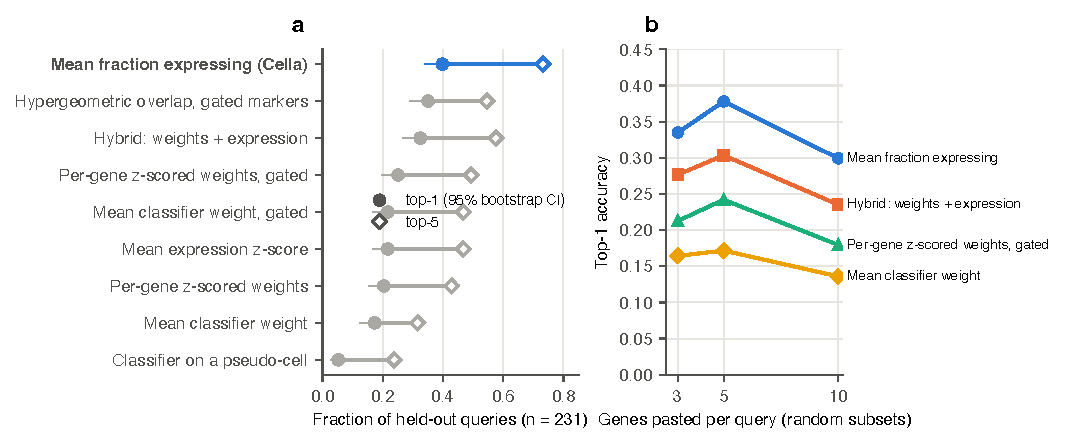
\includegraphics[width=\textwidth]{figures/fig3_lookup.pdf}
\caption{\textbf{Benchmark of signature lookup against external marker sets.} (\textbf{a}) Top-1 (filled, with 95\% bootstrap interval) and top-5 (open) accuracy of nine scoring rules on \lkTest{} independent queries from Tabula Sapiens, Azimuth and PanglaoDB; rules were selected on CellMarker only. (\textbf{b}) Top-1 accuracy when each independent query is reduced to 3, 5 or 10 randomly chosen genes (five draws each).}
\label{fig:lookup}
\end{figure}

\begin{table}[t]
\centering
\small
\caption{\textbf{Lookup benchmark, independent queries.} Development: CellMarker (\lkDev{} queries). Held-out: Tabula Sapiens, Azimuth and PanglaoDB (\lkTest{} queries). MRR, mean reciprocal rank.}
\label{tab:lookup}
\begin{tabular}{@{}lcccc@{}}
\toprule
 & Dev. & \multicolumn{3}{c}{Held-out} \\
\cmidrule(lr){2-2}\cmidrule(lr){3-5}
Scoring rule & Top-1 & Top-1 & Top-5 & MRR \\
\midrule
\tablerows{table_lookup.tex}
\bottomrule
\end{tabular}
\end{table}

\subsection{Gated coefficients make marker panels on par with differential expression}

On cells from datasets that neither method had seen, gated coefficient markers outperformed raw coefficient markers at every panel size and in both readouts (Figure~\ref{fig:panels}). With ten markers per label and classifier-free assignment, gating raised macro-F1 by $\pnMTenRawDiff$ (better in \pnMTenRawWins{} splits, $P = \pnMTenRawP{}$), and by $\pnMTwentyRawDiff$ with twenty markers ($P = \pnMTwentyRawP{}$). Gated coefficients were on par with Wilcoxon markers: the difference was $\pnMTenWilcDiff$ at ten markers ($P = \pnMTenWilcP{}$) and $\pnMTwentyWilcDiff$ at twenty ($P = \pnMTwentyWilcP{}$). They exceeded gated log fold change at ten and twenty markers ($P = \pnMTenLfcP{}$ and $P = \pnMTwentyLfcP{}$). When a classifier was trained on the panel, Wilcoxon markers were better with five markers per label ($\pnLFiveWilcDiff$, $P = \pnLFiveWilcP{}$) and the methods converged at twenty. This readout favours coefficient panels slightly, because their per-label lists overlap less and the union is larger at the same $k$ (\pnSizeGated{} versus \pnSizeWilc{} genes at $k = 10$); the classifier-free readout uses exactly $k$ genes per label and is the fairer comparison. Variation between held-out datasets was large relative to differences between methods (Figure~\ref{fig:panels}), which is why we report paired tests.

\begin{figure}[t]
\centering
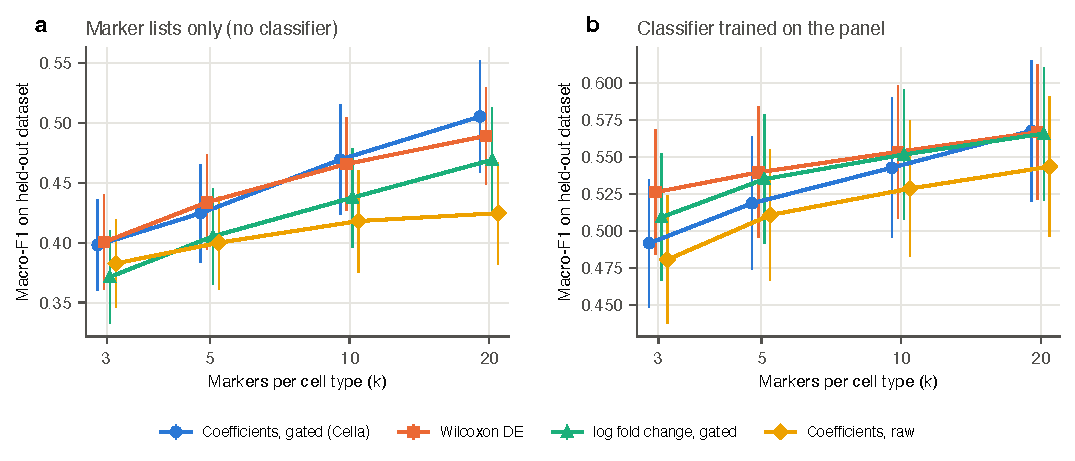
\includegraphics[width=\textwidth]{figures/fig4_panels.pdf}
\caption{\textbf{Marker panels evaluated on held-out datasets.} Macro-F1 on cells of a held-out source dataset (\pnSplits{} splits, \pnOrgans{} organs; mean and 95\% interval across splits) for markers ranked by gated coefficients, Wilcoxon rank-sum, gated log fold change and raw coefficients. (\textbf{a}) Each cell is assigned to the label whose own $k$ markers have the highest mean z-score. (\textbf{b}) A logistic regression is trained on the union of all labels' markers.}
\label{fig:panels}
\end{figure}

\subsection{Use case: organ invariance of discriminative identity}

Comparing a cell type's weight vectors across organs asks whether the same genes distinguish it everywhere. Of \nMultiOrganTerms{} multi-organ terms, \invTierOne{} are annotated at a specific level and \invTierTwo{} coarse terms could be compared on organs in which no subtype was split out (Figure~\ref{fig:invariance}). Calibration mattered: mismatched cell types of two lymphoid organs had a mean cosine of \invNullLL{}, against \invNullPP{} for two peripheral organs, so a single global null would have inflated the scores of cell types compared mostly across blood, bone marrow, spleen and lymph node. With per-pair calibration, circulating lineages remained more organ-invariant than tissue-resident ones (median \invCalCirc{} versus \invCalRes{}; \invNCirc{} versus \invNRes{} terms; one-sided Mann--Whitney $P = \invCalP{}$, compared with $P = \invRawP{}$ before calibration). The difference persisted, more weakly, when only pairs of peripheral organs were used ($P = \invPerP{}$, \invPerNCirc{} versus \invNRes{} terms). It was not explained by the number of cells (Spearman $\rho = \invRhoCells{}$, $P = \invRhoCellsP{}$) or by the reproducibility of the coefficients across disjoint training folds ($\rho = \invRhoStab{}$, $P = \invRhoStabP{}$). This pattern agrees with the established view that tissue environment shapes the identity of resident cells, as shown for macrophage enhancer landscapes \cite{lavin2014} and fibroblast states \cite{buechler2021}. The analysis is small and confined to one atlas collection, and we present it as an example of what the resource makes possible rather than as a definitive result.

\begin{figure}[t]
\centering
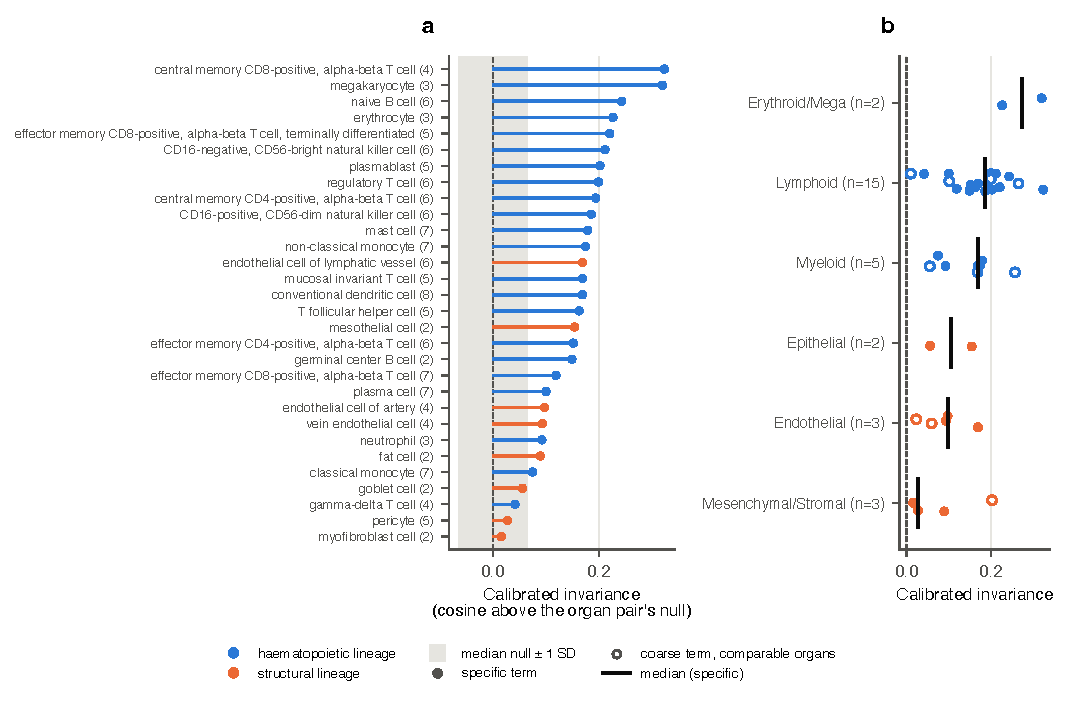
\includegraphics[width=\textwidth]{figures/fig5_invariance.pdf}
\caption{\textbf{Organ invariance of discriminative identity.} (\textbf{a}) Calibrated invariance (mean cross-organ cosine of weight vectors minus each organ pair's mismatched-cell-type null) for the \invTierOne{} specifically annotated terms found in two or more organs; the number of organs is given in parentheses. Blue, circulating lineages; orange, tissue-resident lineages; grey band, typical $\pm 1$ s.d. of a per-pair null. (\textbf{b}) The same scores by lineage, with the median of specific terms; open symbols, coarse terms scored on the organs in which no subtype was annotated.}
\label{fig:invariance}
\end{figure}

\subsection{A serverless deployment that matches the server}

Because the public site has no backend, its answers had to be shown to match those of the service. On \eqQueries{} lookups, comprising the six built-in examples and 120 benchmark queries, the in-browser implementation returned the same top hit as the service for \eqSameTop{}; the remaining \eqTies{} were ties at the precision of the compact tables, where the two best scores differed by less than 0.004. The confidence call agreed for \eqSameConf{} queries, and scores differed by at most \eqMaxDiff{}. Gene-level values agreed to within \eqGeneDiff{} and signature scores to within \eqSigDiff{}, and graph slices, edge details, cell-type search and per-gene cross-organ weights were identical. The site therefore costs nothing to host, has no cold start, and can be archived together with its code and data. One limitation is specific to static mode: classifier weights shown as evidence in lookup hits are available only for genes among the stored top markers, whereas the service reads the full coefficient matrix.

\section{Discussion}

\cella{} makes the classifiers behind a widely used annotation tool readable and queryable without code, and pairs them with the expression summaries needed to interpret them. Two findings shaped the resource and are relevant beyond it. First, coefficients of standardised logistic-regression models should not be ranked directly as markers: rarely detected genes acquire large weights for rare classes, and a simple prevalence gate turns the coefficients into marker lists that perform on par with differential expression on unseen data. That the Wilcoxon test is hard to beat agrees with a systematic comparison of marker-selection methods \cite{pullin2024}; the value of the gated coefficients lies less in outperforming it than in coming from the same model that annotates the data, so that the markers shown are the ones the classifier uses. Second, the classifier's discriminative weights are a poor basis for retrieving a cell type from a short marker list, where expression prevalence does markedly better. Discriminative weights and expression thus answer different questions, and the resource uses each where the benchmarks show it works: weights to describe and compare identity, expression to retrieve it.

Several limitations apply. The resource inherits the scope of the CellTypist organ atlases, including their tissue coverage, annotation granularity and gene vocabularies, and the relationship graph is a similarity graph over weight vectors rather than a reconstruction of the cross-dataset harmonisation of the original work \cite{xu2023}. The lookup benchmark depends on mapping free-text cell-type names to the Cell Ontology and on marker lists that are themselves largely expression-derived, and its accuracy figures should be read as relative rather than absolute. Marker-panel performance varied considerably between held-out datasets, and differential expression retained an advantage in single-nucleus-heavy organs. The invariance analysis rests on \invTierOne{} specifically annotated terms and a single atlas collection; replication in an independent multi-organ atlas profiled from the same donors, such as Tabula Sapiens \cite{tabulasapiens2022}, would be needed to draw biological conclusions.

Future work includes adding further atlases and model releases, recomputing the relationship graph with the original harmonisation approach, and offering programmatic access to the server mode. Because the deployment is static and versioned, each release of \cella{} can be archived and cited as a fixed snapshot.

\section*{Data and code availability}

\cella{} is freely available without registration at \url{https://mdjubayerhossain.com/cella/}. Source code, the analysis and benchmark scripts, the processed artifacts and the scripts that generate every figure and number in this article are available at \url{https://github.com/hossainlab/cella} under the MIT licence. Input data are the public CellTypist organ atlases and models \cite{celltypistorgans}; benchmark queries are public Enrichr libraries \cite{kuleshov2016}. % TODO(author): add Zenodo DOI once archived.

\section*{Funding}

This work received no specific funding.

\section*{Conflict of interest}

None declared.

\section*{Acknowledgements}

We thank the CellTypist developers and the authors of the contributing datasets for making their atlases and models openly available.

\bibliographystyle{unsrtnat}
\bibliography{references}

\end{document}
